%% The first command in your LaTeX source must be the \documentclass command.
\documentclass[sigconf]{acmart}
\begin{document}

\begin{table*}
  \caption{Overview of DNA structural properties and representative variables in protein-DNA interaction.}
  \begin{tabular}{p{5cm}|p{5cm}|p{5cm}|p{1.5cm}}
    \toprule
    DNA structural properties & Facilitated protein-DNA interactions & Representative structural variables & References\\
    \midrule
    DNA stability and propensity for destabilizations and melting bubble formation & Enzymatic processing of substrates, e.g. relaxase nicking of transfer regions\; leads to secondary structure formation & Duplex stability, Thermally induced duplex destabilization (TIDD) & \cite{SantaLucia1998-hc,Lucas2010-gi,Zrimec2015-xf,Sut2009-kg}\\
    Major and minor groove properties & Readout of chemical information, e.g. transcription factors in promoters & DNAShape, ORChID2 & \cite{Rohs2009-hm,Chiu2016-kb,Bishop2011-jm,Watson2008-dt}\\
    Intrinsically curved or flexible regions & Binding and topological changes, e.g. IHF binding in promoters & DNAzeI cleavage frequency, Persistence length & \cite{Brukner1995-pt,Geggier2010-mw,Moncalian1999-qj}\\
    DNA twist and supercoiling & Topological changes recognized by proteins, e.g. histones, and affect multiple other properties & Twist and other conformational variables & \cite{Karas1996-qz,Olson1998-rw,Perez2004-sx,Watson2008-dt}\\
    Differences in DNA spacing and orientation in binding and enzymatic sites & Affect binding with multiple contact points and protein complex formation & Helical repeats & \cite{Williams2007-be,Geggier2010-mw,Watson2008-dt}\\
    Propensity for transitions between DNA forms B-DNA, A-DNA, Z-DNA & Affect overall features recognized by proteins and their accessibility & B-A and B-Z transition propensities & \cite{Aida1988-iq,Ho1986-hg,Hartmann1989-ji,Kulkarni2013-xm}\\
    \bottomrule
  \end{tabular}
\end{table*}

\begin{figure*}[ht]
  \centering
  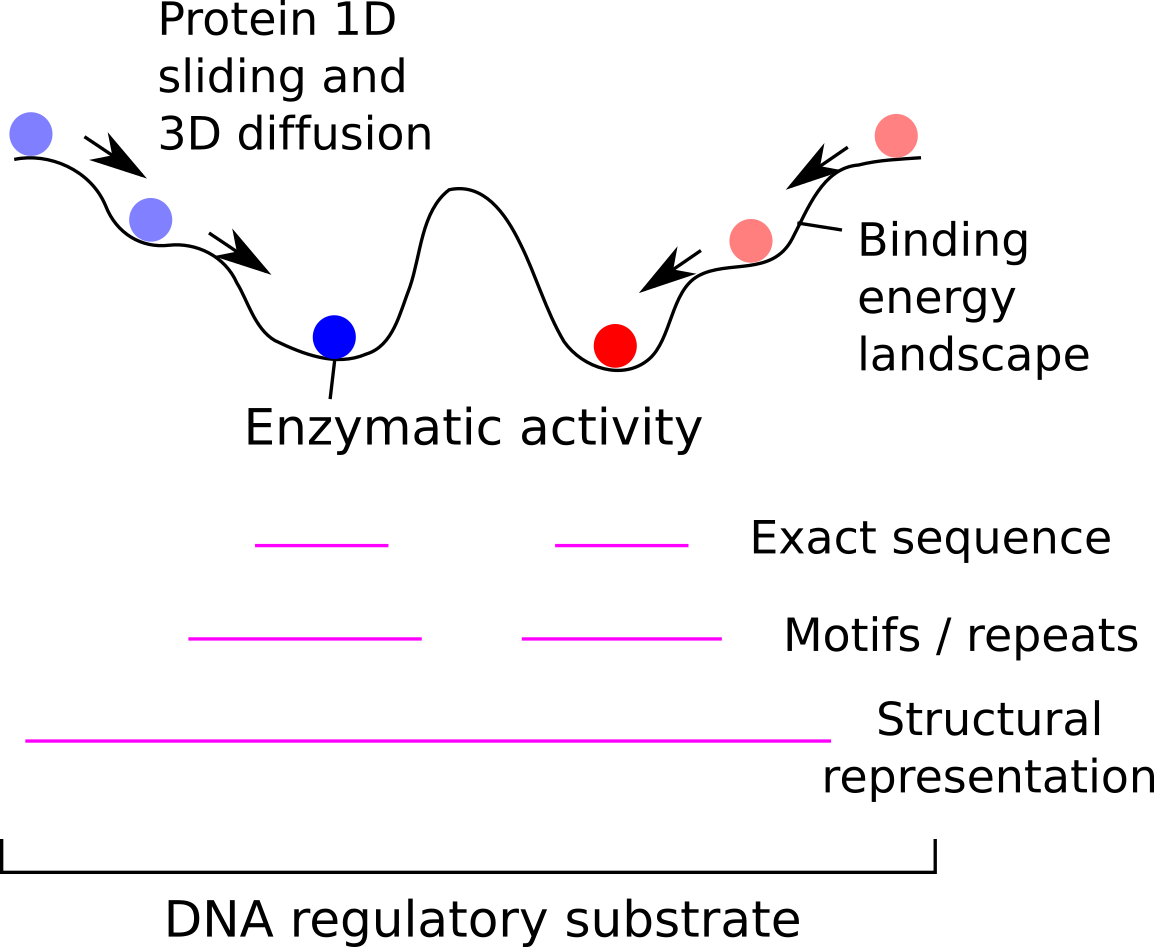
\includegraphics[width=6cm,keepaspectratio]{smir_fig_algorithms.png}
  \caption{Possibilities for combined sequence structure algorithms based on how proteins recognize and bind their active sites in the regulatory DNA \cite{Marcovitz2013-kg,Levo2015-iu,Slattery2014-ne,Rohs2009-hm}. Interactions of lower specificity with the surrounding DNA (corresponding to DNA with less conserved nucleotide sequence but defined structural properties) guide the proteins towards their specific binding sites (highly conserved or exact sequence).}
\end{figure*}

\bibliographystyle{jphysicsB}
\bibliography{References_C4A_acm-bcb-20_BibTeX}

\end{document}